\documentclass[10pt,a4paper,titlepage]{article}
\usepackage[utf8]{inputenc}
\usepackage{amsmath}
\usepackage{amsfonts}
\usepackage{amssymb}
\usepackage{graphicx}
\usepackage{lmodern}
\usepackage{xcolor}
\usepackage{qtree}
\usepackage{listings}
\usepackage{color}
\usepackage[xetex, hypertexnames=false, breaklinks=true, pdfborder={0 0 0},
pdfauthor={Timo Homburg},
pdftitle={J2Latex Projectdescription},
pdfsubject={J2Latex},
pdfkeywords={Java,LaTeX,HTML,Compiler,JavaCC},
pdfproducer={Xetex with hyperref},
pdfcreator={Pdflatex}]{hyperref}
\definecolor{gray}{rgb}{0.4,0.4,0.4}
\definecolor{darkblue}{rgb}{0.0,0.0,0.6}
\definecolor{cyan}{rgb}{0.0,0.6,0.6}
\lstset{
basicstyle=\footnotesize,
frame=single,,
  columns=fullflexible,
  showstringspaces=false,
  commentstyle=\color{gray}\upshape,
  keepspaces
                 % Linienstaerke des Rahmens
}
\lstdefinelanguage{XML}
{
  morestring=[b]",
  morestring=[s]{>}{<},
  morecomment=[s]{<?}{?>},
  stringstyle=\color{black},
  identifierstyle=\color{darkblue},
  keywordstyle=\color{cyan},
  morekeywords={xmlns,version,type}% list your attributes here
}
\begin{document}
\textbf{\large J2Latex Documentation}\\\ \\\\\\\
The goal of the project has been to write a compiler which would take a Java class a produces a nicely formatted LaTeX or HTML document of it.
To achieve this goal a Java grammar has been implemented using JavaCC and two Visitorclasses (asLatex.java, asHTML.java) have been created. The project does not cover every feature of the Java language and can be extended to support more features in the future.
The following features have been implemented:\begin{itemize}
	\item All Operators
	\item All Keywords
	\item Typecasts
	\item If/ElseIf/Else
	\item Switch/Case/Default
	\item Exceptions(Try/Catch/Finally und Throw/Throws)
	\item Class definitions
	\item Anonymous inner classes
	\item Interfaces
	\item Functions
	\item Class variables
	\item Constant values
	\item Hex,Oct and Decimalconstants
	\item String and Charconstants
	\item Extends/Implements
	\item Generics (only single generics)
	\item Function annotations (@Override)
	\item Imports
	\item Packetdefinitions
	\item Enum and Enumclasses
	\item Constructors including super()
\end{itemize}
Sample classes for testing are provided in the sample package of the project. All classes in this package are valid Java classes and covered aforementioned features. To start the program, the class Test.java needs to be executed and will produce one output in HTML and LaTeX/PDF respectively. In figure \ref{j2latextree} the parsetree of the application is shown:
\begin{figure}
	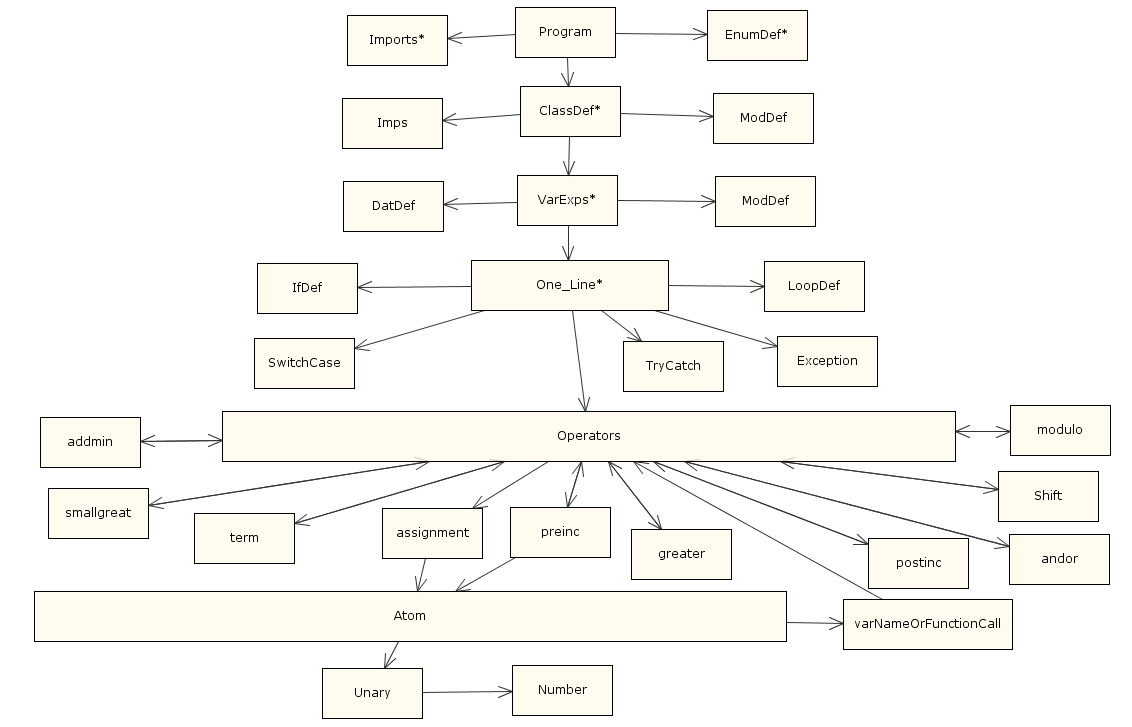
\includegraphics[width=1.3\linewidth]{img/parsetree.png}
	\caption{J2Latex Parsetree}
	\label{j2latextree}
\end{figure}

\end{document}